% Figure s05f01_flux (Session 5): flux quantization as a macroscopic readout of h/2e.
% The image is rendered by figures/blender/s05f01_flux.py; the coordinates of the labels come from
% figures/blender/out/s05f01_flux_anchors.tex. Build with figures/blender/build_figure.sh s05f01_flux.
\documentclass[11pt,tikz,border=0pt]{standalone}
\usepackage[T1]{fontenc}
\usepackage{amsmath,amssymb,graphicx,bm}
\usepackage{xcolor}
\usetikzlibrary{arrows.meta,calc}
% The three label colors of the figures, with the same values as in src/figures_preamble.tex.
\definecolor{aqmaccent}{RGB}{31,78,121}
\definecolor{aqmbroken}{RGB}{168,42,34}
\definecolor{aqmmuted}{RGB}{125,125,125}

\newlength{\figw}\setlength{\figw}{10.9cm}   % 0.70 of the text width, before the empty margins of the render are cropped

\begin{document}
\begin{tikzpicture}[lbl/.style={font=\small, inner sep=1.5pt}, pnl/.style={font=\small\bfseries, inner sep=1.5pt}]
  \begin{scope}
    \setlength{\figw}{5.3cm}
    \node[overlay, anchor=south west, inner sep=0pt] at (0,0)
      {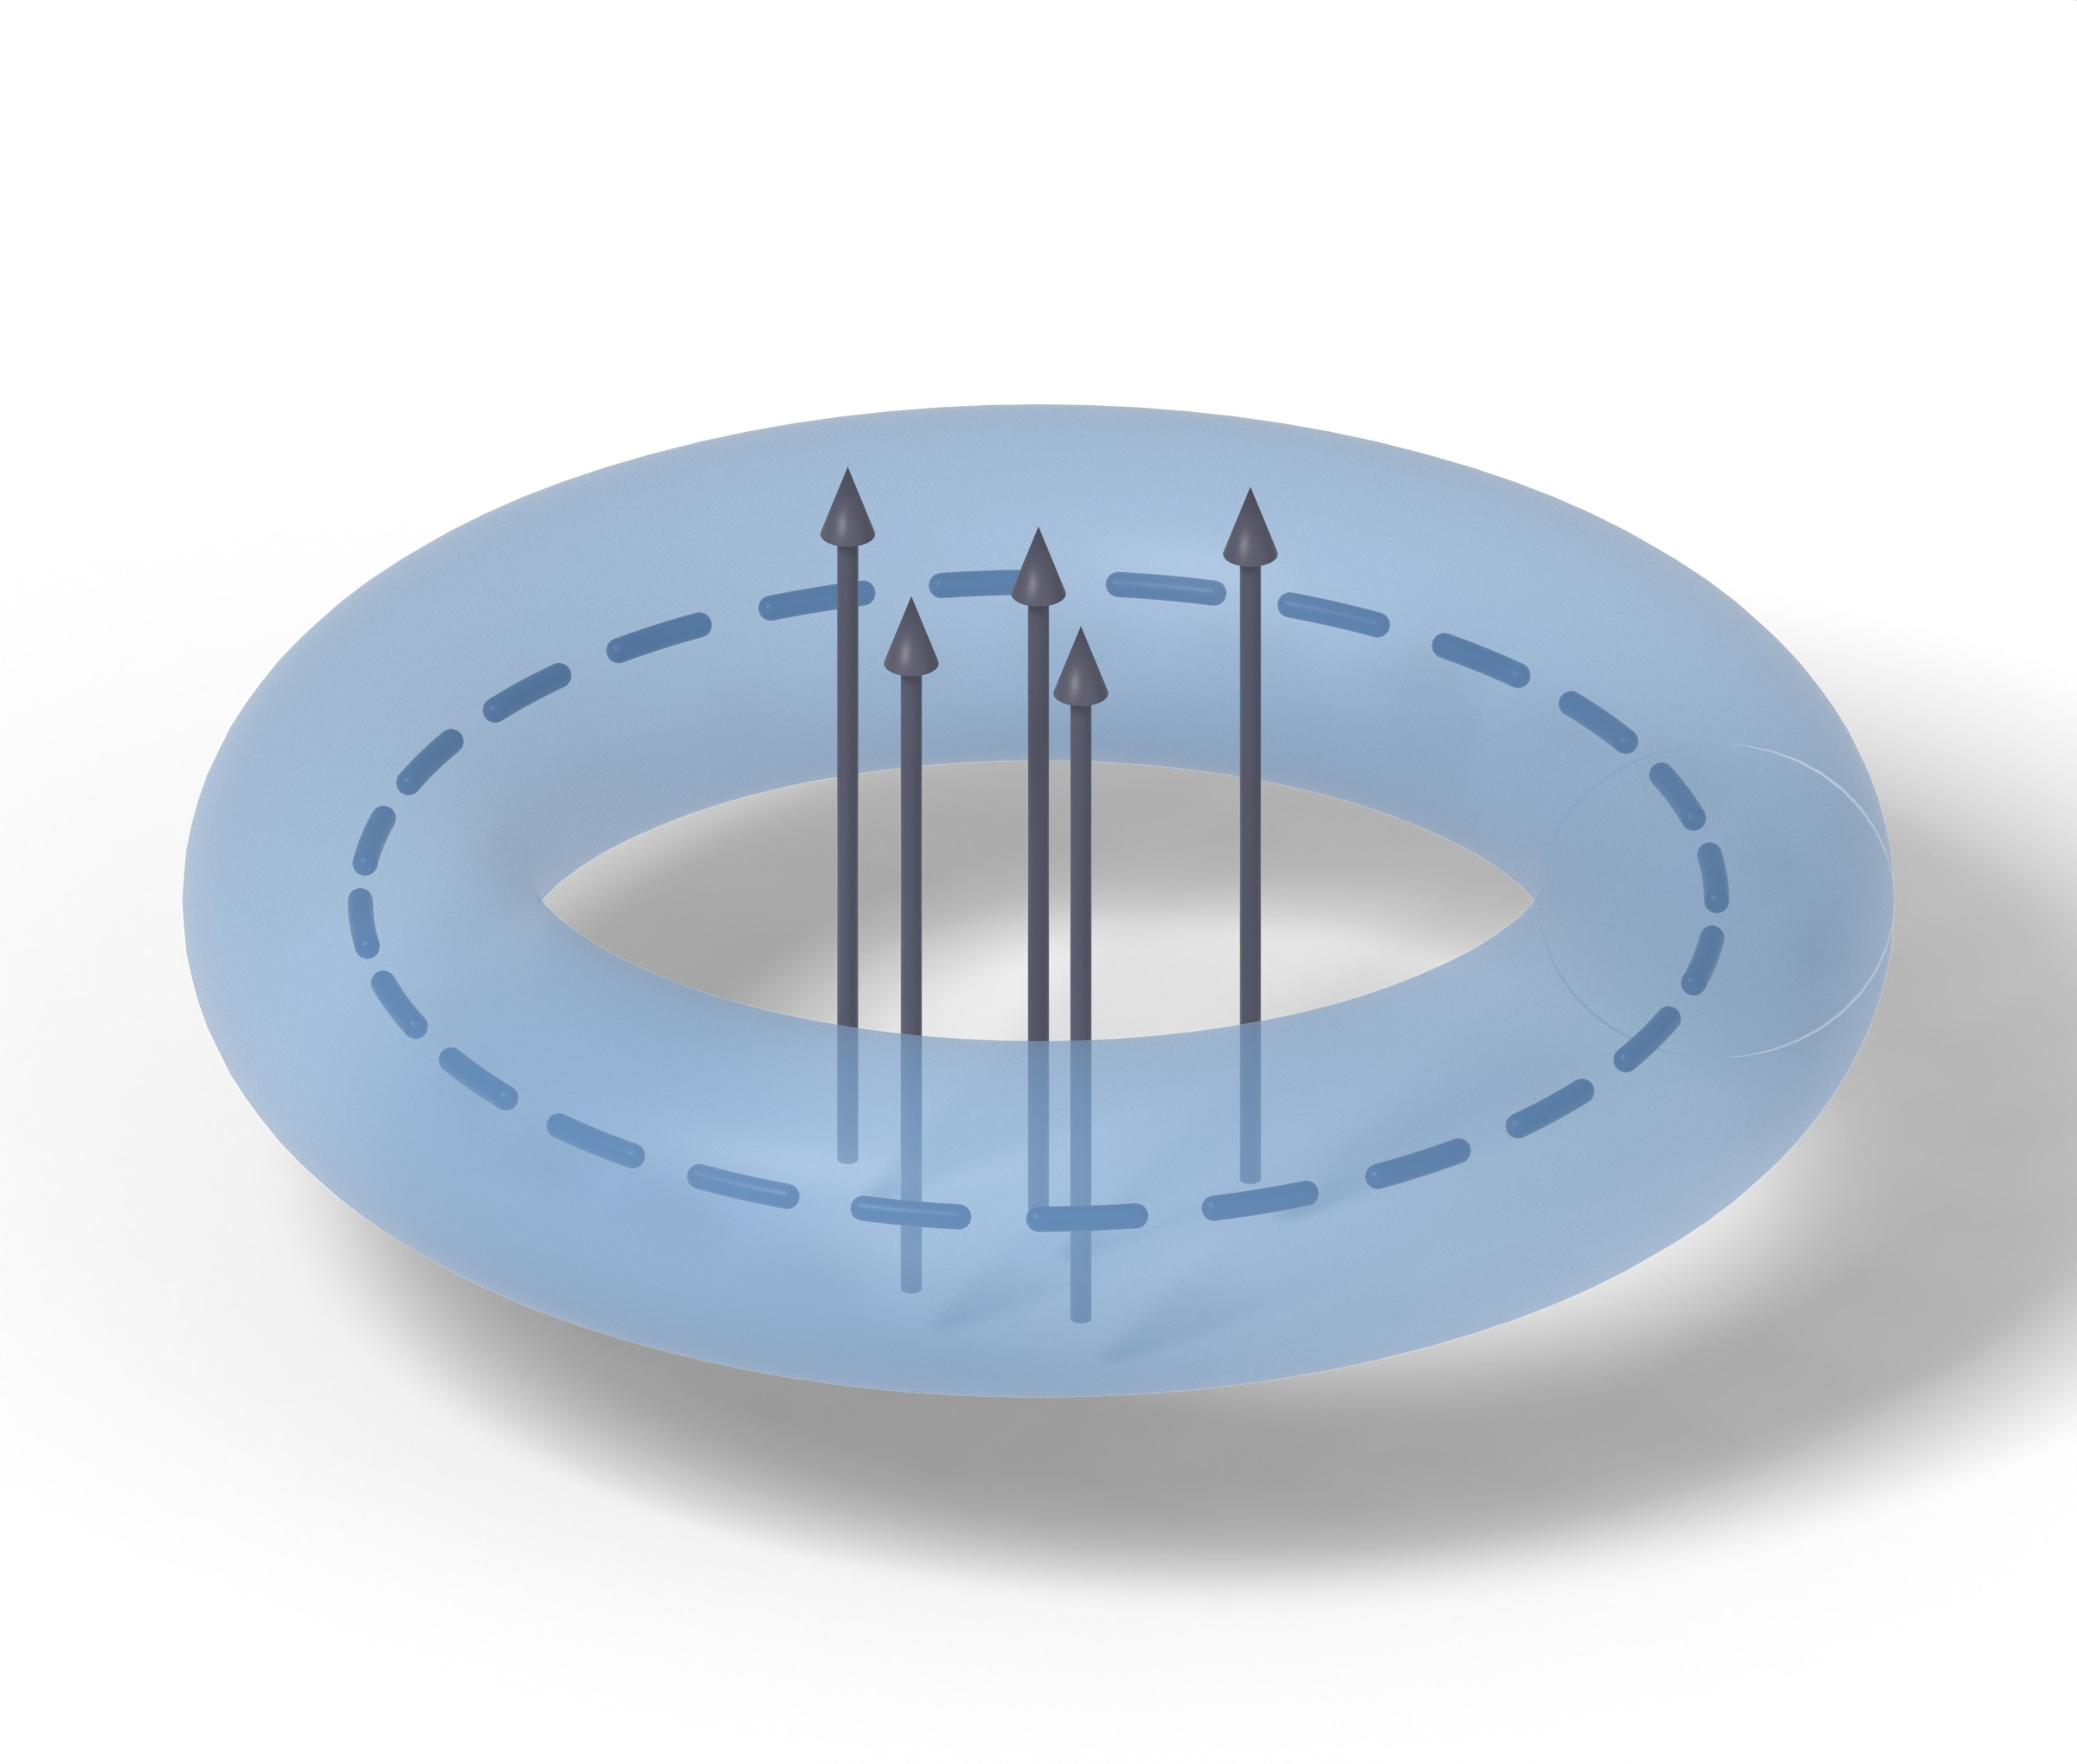
\includegraphics[width=\figw]{../blender/out/s05f01_flux_a.jpg}};
    % written by build_figure.sh; the painted part of the image
\path (0.0200\figw,0.0688\figw) rectangle (0.9988\figw,0.6550\figw);

    %% written by figlib.py; x and y in units of the image width
\coordinate (aPhi) at (0.5204\figw,0.6138\figw);
\coordinate (acontour) at (0.7030\figw,0.2108\figw);
\coordinate (apanel) at (0.0469\figw,0.6498\figw);

    \node[lbl, anchor=south, yshift=2pt] at (aPhi) {$\Phi=n\,h/2e$};
    \node[lbl, anchor=north, text=aqmaccent, align=center] at (acontour) {$\hbar\nabla\theta=2e\mathbf A$};
  \end{scope}
  \begin{scope}[shift={(5.5cm,0)}]
    \setlength{\figw}{5.4cm}
    \node[overlay, anchor=south west, inner sep=0pt] at (0,0)
      {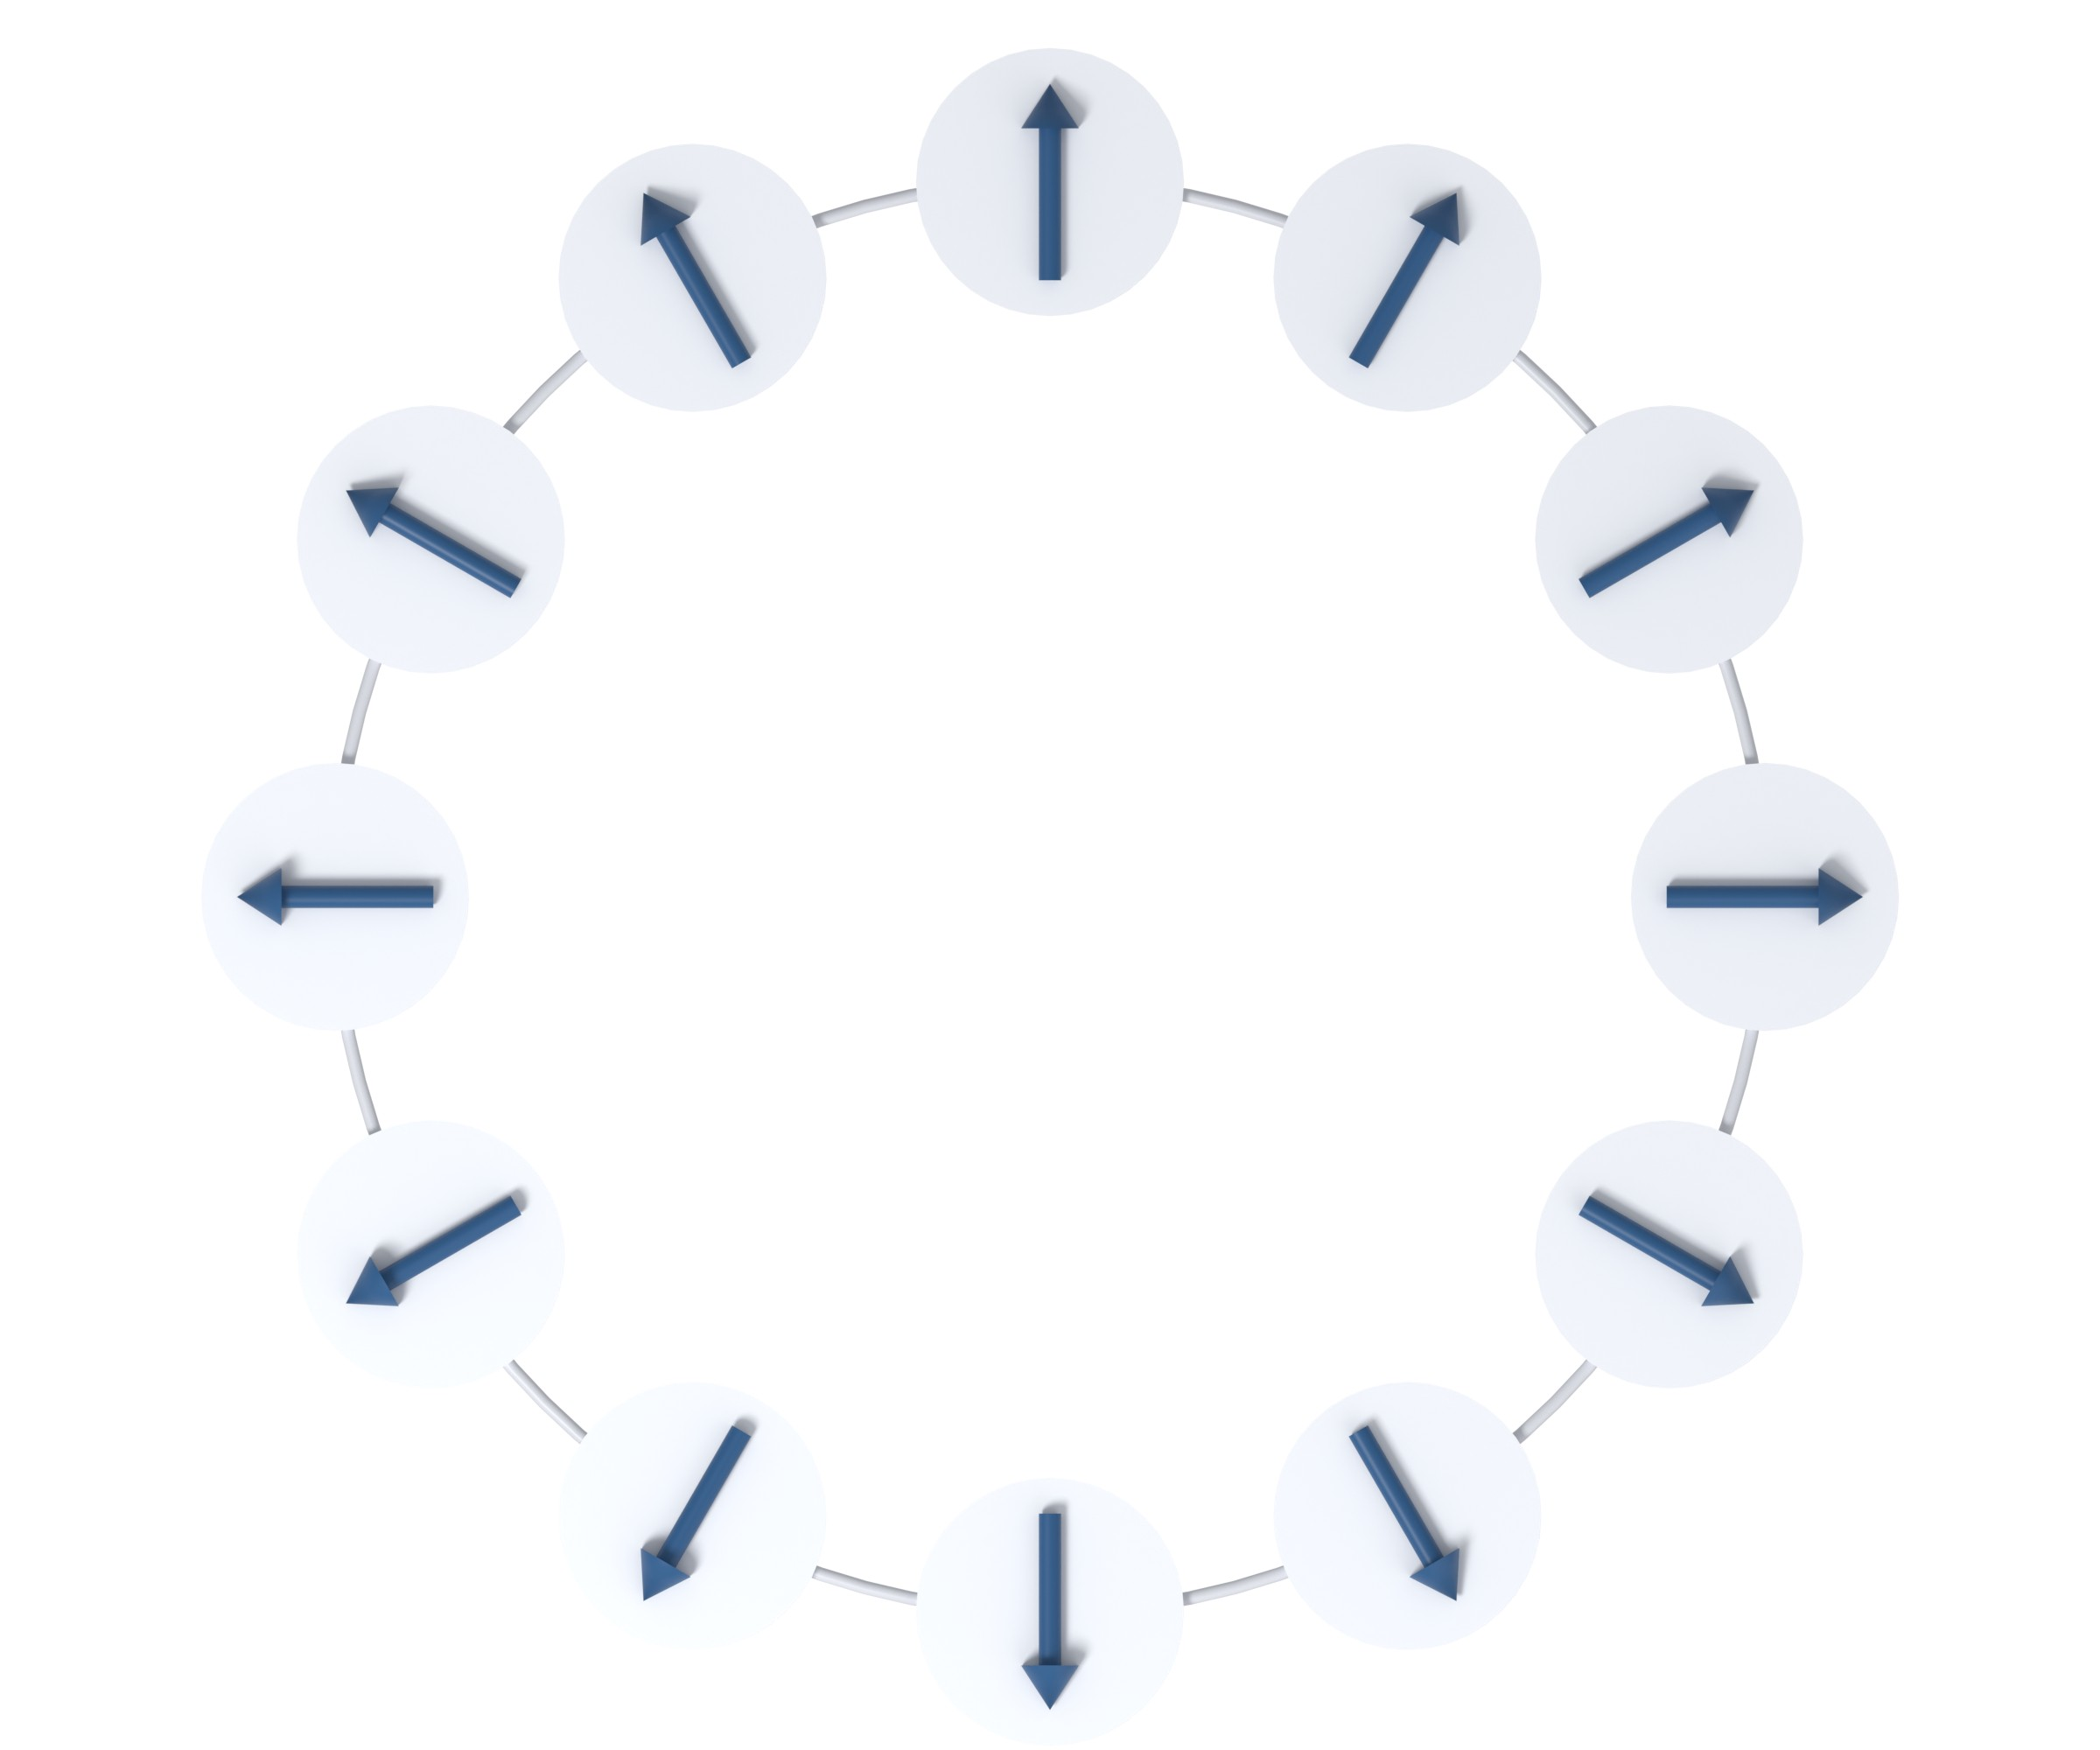
\includegraphics[width=\figw]{../blender/out/s05f01_flux_b.jpg}};
    % written by build_figure.sh; the painted part of the image
\path (0.0958\figw,0.0050\figw) rectangle (0.9042\figw,0.8104\figw);

    %% written by figlib.py; x and y in units of the image width
\coordinate (bstart) at (0.9149\figw,0.4062\figw);
\coordinate (bcenter) at (0.5000\figw,0.4062\figw);
\coordinate (bpanel) at (0.0000\figw,0.8424\figw);

    \node[lbl, align=center] at (bcenter) {$\theta$ winds\\by $2\pi n$};
  \end{scope}
\end{tikzpicture}
\end{document}
